\documentclass[preprint,12pt]{elsarticle}

\usepackage{amsmath,amssymb,amsthm}
\usepackage{booktabs}
\usepackage{graphicx}
\usepackage{hyperref}

\newtheorem{theorem}{Theorem}
\newtheorem{proposition}{Proposition}
\newtheorem{lemma}{Lemma}
\newtheorem{corollary}{Corollary}
\newtheorem{remark}{Remark}

\journal{Journal of Computational Physics}

\begin{document}

\begin{frontmatter}

\title{Exactness-preserving discrete Maxwell operators\\on periodic polyhedral complexes}

\author{Alex Toader}
\address{Independent researcher}

\begin{abstract}
\emph{Problem.}
The standard Bloch-periodic extension of discrete exterior calculus (DEC) on unstructured polyhedral meshes breaks the discrete de~Rham exact sequence: $d_1(\mathbf{k})\,d_0(\mathbf{k}) \neq 0$ for generic wave vector~$\mathbf{k}$. This failure produces spectral pollution in the curl--curl eigenvalue problem, compromises the discrete Hodge splitting, and prevents convergence of the acoustic dispersion relation.
%
\emph{Construction.}
We build an exactness-preserving $d_1(\mathbf{k})$ via a face-boundary recurrence that derives the Bloch phases from those already present in the gradient $d_0(\mathbf{k})$. No per-edge phase assignment independent of $d_0(\mathbf{k})$ can achieve exactness on a generic unstructured mesh. The construction is unique up to a $U(1)$ phase per face, and the curl--curl operator $K(\mathbf{k}) = d_1(\mathbf{k})^\dagger\,\star_2\,d_1(\mathbf{k})$ is canonical.
%
\emph{Results.}
Verification on five periodic polyhedral complexes---including Voronoi foams and random meshes---confirms that exactness eliminates the pollution, restores the Hodge decomposition, and yields acoustic dispersion with second-order dispersion error $O((ka)^2)$ and clean band structure across the full Brillouin zone. The exact complex computes the twisted de~Rham cohomology $H^*(T^3, \mathcal{L}_\mathbf{k})$: Betti numbers $(1,3,3,1)$ at $\Gamma$ and $(0,0,0,0)$ at $\mathbf{k} \neq 0$. The standard construction, not being a cochain complex, cannot define cohomology.
\end{abstract}

\begin{keyword}
discrete exterior calculus \sep Bloch boundary conditions \sep Maxwell eigenvalues \sep polyhedral meshes \sep de~Rham exactness \sep spectral pollution \sep twisted cohomology
\end{keyword}

\end{frontmatter}

% ------------------------------------------------------------------
\section{Introduction}
\label{sec:intro}
% ------------------------------------------------------------------

The discrete exterior calculus (DEC) provides a coordinate-free discretization of differential forms on cell complexes~\cite{Hirani2003,Desbrun2005}. For Maxwell's equations on periodic structures, DEC represents the electric field as a 1-cochain (edge values) and the magnetic flux as a 2-cochain (face values), with discrete gradient~$d_0$ and curl~$d_1$ acting between cochain spaces. The curl--curl eigenvalue problem
\begin{equation}\label{eq:curlcurl}
  K\,\mathbf{a} = \omega^2 M\,\mathbf{a}, \qquad
  K = d_1^\dagger \star_2\, d_1, \qquad M = \star_1
\end{equation}
yields electromagnetic eigenfrequencies when the discrete de~Rham sequence
\begin{equation}\label{eq:derham}
  C^0 \xrightarrow{d_0} C^1 \xrightarrow{d_1} C^2
\end{equation}
is exact, i.e., $d_1\,d_0 = 0$. Boffi~\cite{Boffi2010} established that exactness of the discrete complex is necessary and sufficient for spurious-free Maxwell eigenvalue computations: without it, the gauge kernel is incomplete and spectral pollution is unavoidable.

For periodic structures, Bloch boundary conditions twist the operators by a wave vector $\mathbf{k} \in \mathbb{R}^3$. On structured grids (Yee lattice), this is straightforward: the uniform topology ensures $d_1(\mathbf{k})\,d_0(\mathbf{k}) = 0$ automatically. However, on unstructured polyhedral meshes---as arise from Voronoi tessellations of periodic point sets---the standard construction of applying independent Bloch phases to each entry of~$d_1$ breaks exactness at $\mathbf{k} \neq 0$. The core difficulty is not the twisting itself---twisted cochain complexes and flat local systems are classical~\cite{Bott1982}---but the incompatibility between independent edge-based phase lifting and the face-wise exactness constraints on non-tensorial meshes. On structured grids, the tensor-product topology ensures pairwise cancellation at every face. On unstructured meshes, the face boundaries mix edges with heterogeneous lattice shifts, and no per-edge phase assignment independent of $d_0(\mathbf{k})$ can restore exactness (Corollary~\ref{cor:noedge}).

The preservation of discrete exactness for Bloch-periodic DEC operators on general polyhedral meshes does not appear to have been treated explicitly in the literature. Existing DEC-based Maxwell computations use either structured grids where the issue does not arise~\cite{Teixeira1999}, or non-periodic domains where Bloch conditions are unnecessary~\cite{Chen2017}. The discrete de~Rham (DDR) method~\cite{DiPietro2020} achieves exactness on polyhedral meshes but has not been formulated with Bloch periodicity. The mimetic finite difference method of Jin, Xia, and Xu~\cite{Jin2025} treats Bloch boundary conditions on structured meshes but does not consider the unstructured case. Band structure computations on foam-like structures~\cite{Klatt2019} use plane-wave expansion, not DEC.

\paragraph{Contribution} We present:
\begin{enumerate}
  \item An explicit construction of an exactness-preserving $d_1(\mathbf{k})$ via a recurrence that derives the curl phases from those already present in $d_0(\mathbf{k})$, exploiting the flat holonomy of the Bloch connection on each face (\S\ref{sec:construction}).
  \item A proof that $d_1(\mathbf{k})$ is unique up to a $U(1)$ phase per face, and that the curl--curl operator $K(\mathbf{k})$ is canonical (\S\ref{sec:construction}).
  \item A systematic demonstration that the standard Bloch extension produces spectral pollution that enters the physical spectrum, destroys the Hodge splitting, and does not converge under mesh refinement (\S\ref{sec:consequences}).
  \item Numerical verification on five qualitatively different periodic polyhedral complexes, including random Voronoi meshes with no symmetry (\S\ref{sec:consequences}--\ref{sec:robustness}).
  \item Computation of the twisted de~Rham cohomology $H^p(T^3, \mathcal{L}_\mathbf{k})$ via the exact complex, yielding Betti numbers $(1,3,3,1)$ at~$\Gamma$ and $(0,0,0,0)$ at generic~$\mathbf{k}$, with a physical interpretation: the three harmonic 1-forms at~$\Gamma$ deform into one longitudinal gradient mode and two transverse acoustic modes at small~$|\mathbf{k}|$ (\S\ref{sec:cohomology}).
\end{enumerate}
Items~(1)--(2) are mathematically new: the exactness failure of the standard Bloch extension on unstructured meshes has not, to our knowledge, been previously identified, and the face-boundary recurrence that corrects it is a new construction. Items~(3)--(4) provide the first numerical evidence that this structural error produces spectral pollution, broken Hodge splitting, and convergence failure on realistic foam geometries. Item~(5) demonstrates that the exact complex computes the correct sheaf cohomology and connects the topological invariants to the band structure.

% ------------------------------------------------------------------
\section{Periodic complexes and DEC operators}
\label{sec:setup}
% ------------------------------------------------------------------

\subsection{Cell complex on the torus}

Let $\Lambda = L_x\mathbb{Z} \times L_y\mathbb{Z} \times L_z\mathbb{Z}$ be a lattice in $\mathbb{R}^3$ with fundamental domain $\Omega = [0,L_x) \times [0,L_y) \times [0,L_z)$. A periodic cell complex $(V, E, F, C)$ on the flat torus $T^3 = \mathbb{R}^3/\Lambda$ consists of vertices~$V$, oriented edges~$E$, oriented faces~$F$, and 3-cells~$C$.

Edges connecting vertices across the periodic boundary carry a lattice shift vector $\mathbf{n}_e \in \mathbb{Z}^3$:
\begin{equation}\label{eq:shift}
  \mathbf{n}_e = \operatorname{round}\!\bigl((\mathbf{x}_j - \mathbf{x}_i) / \mathbf{L}\bigr)
\end{equation}
where division is componentwise. Interior edges have $\mathbf{n}_e = \mathbf{0}$.

\subsection{Incidence matrices}

The topological gradient $d_0 \in \mathbb{R}^{|E|\times|V|}$ and curl $d_1 \in \mathbb{R}^{|F|\times|E|}$ encode the boundary relations:
\begin{equation}\label{eq:d0}
  (d_0)_{ev} = \begin{cases}
    +1 & \text{if } v = \operatorname{head}(e), \\
    -1 & \text{if } v = \operatorname{tail}(e), \\
    \phantom{+}0  & \text{otherwise},
  \end{cases}
\end{equation}
\begin{equation}\label{eq:d1}
  (d_1)_{fe} = \begin{cases}
    +1 & \text{if } e \in \partial f,\ \text{same orientation}, \\
    -1 & \text{if } e \in \partial f,\ \text{opposite orientation}, \\
    \phantom{+}0  & \text{if } e \notin \partial f.
  \end{cases}
\end{equation}
These satisfy $d_1 d_0 = 0$ (every vertex appears in the boundary of a face an even number of times with canceling signs).

\subsection{Hodge stars}

The diagonal Hodge star operators $\star_1 \in \mathbb{R}^{|E|\times|E|}$ and $\star_2 \in \mathbb{R}^{|F|\times|F|}$ encode metric information from the dual complex:
\begin{equation}\label{eq:stars}
  (\star_1)_{ee} = \frac{|\sigma^*_e|}{|\sigma_e|}, \qquad
  (\star_2)_{ff} = \frac{|\sigma^*_f|}{|\sigma_f|}
\end{equation}
where $\sigma_e$, $\sigma_f$ are primal edge length and face area, and $\sigma^*_e$, $\sigma^*_f$ are their dual counterparts. For the SC cubic benchmark with lattice constant~$a$, the stars are uniform: $\star_1 = a\,I$, $\star_2 = a^{-1}\,I$.

\subsection{Test structures}
\label{sec:structures}

We verify the construction on five periodic polyhedral complexes spanning three qualitatively different categories.

\begin{table}[h]
\centering
\begin{tabular}{llrrrcc}
\toprule
Structure & Type & $|V|$ & $|E|$ & $|F|$ & Plateau & $O_h$ \\
\midrule
SC cubic ($N{=}3$) & regular lattice & 27  & 81  & 81  & no  & yes \\
C15 (Laves)        & Voronoi foam   & 136 & 272 & 160 & yes & yes \\
Kelvin (BCC)       & Voronoi foam   & 96  & 192 & 112 & yes & yes \\
Weaire--Phelan     & Voronoi foam   & 46  & 92  & 54  & yes & yes \\
Random Voronoi     & random         & 206--354 & 412--708 & 236--404 & yes & no  \\
\bottomrule
\end{tabular}
\caption{Test structures. Plateau foams have 4 edges per vertex and 3 faces per edge. The random Voronoi complexes are constructed from 50 uniformly distributed points; the range reflects 10 different seeds.}
\label{tab:structures}
\end{table}

\begin{figure}[h]
\centering
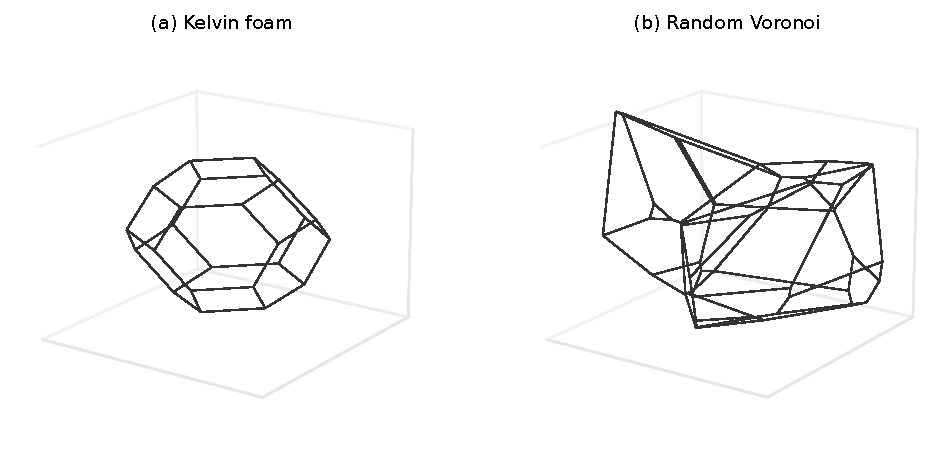
\includegraphics[width=\textwidth]{fig3_meshes_m5.pdf}
\caption{Wireframe view of two test structures (central region of the periodic box). (a)~Kelvin foam: regular BCC Voronoi tessellation producing truncated octahedra with hexagonal and square faces. (b)~Random Voronoi: irregular polyhedral cells with no lattice symmetry. The full periodic complexes used in the computations contain $|V| = 96$--$354$ vertices (Table~\ref{tab:structures}).}
\label{fig:meshes}
\end{figure}

% ------------------------------------------------------------------
\section{The exactness problem}
\label{sec:problem}
% ------------------------------------------------------------------

\subsection{Bloch-twisted gradient}

For wave vector $\mathbf{k} \in \mathbb{R}^3$, the Bloch-twisted gradient is (where $\mathbf{n}_e\mathbf{L}$ denotes the componentwise product $(n_{e,1}L_x,\, n_{e,2}L_y,\, n_{e,3}L_z)$):
\begin{equation}\label{eq:d0k}
  d_0(\mathbf{k})[e,v] = \begin{cases}
    +e^{i\mathbf{k}\cdot\mathbf{n}_e\mathbf{L}} & \text{if } v = \operatorname{head}(e), \\
    -1 & \text{if } v = \operatorname{tail}(e), \\
    \phantom{+}0 & \text{otherwise}.
  \end{cases}
\end{equation}
This is standard and well-defined: each edge carries a unique lattice shift. The asymmetric placement of the phase on the head vertex is a gauge choice; any other convention (e.g., symmetric $e^{\pm i\mathbf{k}\cdot\mathbf{n}_e\mathbf{L}/2}$) is related by a vertex-based gauge transform $u_v \mapsto e^{i\theta(v)}u_v$ and yields the same physical spectrum.

\subsection{Standard Bloch curl}

The standard extension applies independent Bloch phases per face:
\begin{equation}\label{eq:d1std}
  d_1^{\mathrm{std}}(\mathbf{k})[f,e] = d_1[f,e] \cdot e^{i\mathbf{k}\cdot\mathbf{n}_e\mathbf{L}}.
\end{equation}
On tensor-product (structured) grids, this preserves exactness: each face is a quadrilateral whose opposite edges carry identical lattice shifts, so the Bloch phases cancel pairwise at every vertex. On unstructured meshes, faces generically have boundary edges with heterogeneous shifts, and exactness fails.

\subsection{Diagnosis}

The product $d_1(\mathbf{k})\,d_0(\mathbf{k})$ at a face~$f$ and vertex~$v$ yields
\begin{equation}\label{eq:product}
  (d_1 d_0)[f,v] = \sum_{\substack{e \in \partial f \\ v \in e}} d_1(\mathbf{k})[f,e] \cdot d_0(\mathbf{k})[e,v].
\end{equation}
At $\mathbf{k} = \mathbf{0}$, cancellation is guaranteed by the topological constraint $d_1 d_0 = 0$. At $\mathbf{k} \neq \mathbf{0}$, the phases on different boundary edges prevent cancellation unless they are mutually consistent.

\begin{proposition}[Standard construction breaks exactness]\label{prop:break}
Let $f$ be a face with at least two boundary edges $e_a$, $e_b$ sharing a vertex and having distinct lattice shifts $\mathbf{n}_a \neq \mathbf{n}_b$. Then $d_1^{\mathrm{std}}(\mathbf{k})\,d_0(\mathbf{k}) \neq 0$ for almost all $\mathbf{k} \in \mathbb{R}^3$.
\end{proposition}

\begin{proof}
At the shared vertex~$v$, the two contributions carry phases $e^{i\mathbf{k}\cdot\mathbf{n}_a\mathbf{L}}$ and $e^{i\mathbf{k}\cdot\mathbf{n}_b\mathbf{L}}$. Cancellation requires $e^{i\mathbf{k}\cdot(\mathbf{n}_a - \mathbf{n}_b)\mathbf{L}} = 1$, which defines a hyperplane in $\mathbf{k}$-space. This holds at $\mathbf{k} = \mathbf{0}$ but fails generically when $\mathbf{n}_a \neq \mathbf{n}_b$.
\end{proof}

More generally, the failure is not specific to the standard phase choice:

\begin{corollary}[No per-edge phase assignment suffices]\label{cor:noedge}
Let $\varphi\colon\mathbb{Z}^3\to\mathbb{C}^*$ be any function of the lattice shift. Define $\tilde{d}_1(\mathbf{k})[f,e] = d_1[f,e]\cdot\varphi(\mathbf{n}_e,\mathbf{k})$. If the complex contains a face~$f$ with two boundary edges $e_a$, $e_b$ satisfying $\mathbf{n}_{e_a} = \mathbf{n}_{e_b}$ and separated along $\partial f$ by an edge~$e_c$ with $\mathbf{n}_{e_c} \neq \mathbf{n}_{e_a}$, then $\tilde{d}_1(\mathbf{k})\,d_0(\mathbf{k}) \neq 0$ for generic~$\mathbf{k}$.
\end{corollary}

\begin{proof}
By Corollary~\ref{cor:unique}, any $d_1(\mathbf{k})$ satisfying $d_1\,d_0 = 0$ has $d_1[f,:] = \lambda_f\cdot d_1^{\mathrm{ex}}[f,:]$ for some $\lambda_f$, where $d_1^{\mathrm{ex}}$ is the recurrence construction with phases $\psi_0, \ldots, \psi_{n-1}$.

The per-edge hypothesis gives $\tilde{d}_1[f, e_a] = \sigma_a\,\varphi(\mathbf{n}_{e_a})$ and $\tilde{d}_1[f, e_b] = \sigma_b\,\varphi(\mathbf{n}_{e_b})$. If $\tilde{d}_1\,d_0 = 0$, equating with the unique exact solution:
\begin{equation}\label{eq:peredge}
  \varphi(\mathbf{n}_{e_a}) = \lambda_f\,\psi_a, \qquad \varphi(\mathbf{n}_{e_b}) = \lambda_f\,\psi_b.
\end{equation}
Since $\mathbf{n}_{e_a} = \mathbf{n}_{e_b}$, we need $\psi_a = \psi_b$. However, the recurrence gives
\begin{equation}\label{eq:phaseproduct}
  \psi_b / \psi_a = \prod_{i=a+1}^{b} \frac{-\sigma_{i-1}\,d_0(\mathbf{k})[e_{i-1}, v_i]}{\sigma_i\,d_0(\mathbf{k})[e_i, v_i]}
  = e^{i\mathbf{k}\cdot\mathbf{S}_{a\to b}\mathbf{L}}
\end{equation}
where $\mathbf{S}_{a\to b} \in \mathbb{Z}^3$ is an integer vector determined by the lattice shifts and orientations of the intervening edges (each factor contributes $e^{i\mathbf{k}\cdot\boldsymbol{\alpha}_i\mathbf{L}}$ with $\boldsymbol{\alpha}_i \in \{\mathbf{n}_{i-1},\, \mathbf{n}_{i-1}{-}\mathbf{n}_i,\, \mathbf{0},\, {-}\mathbf{n}_i\}$ depending on the signs $\sigma_{i-1}, \sigma_i$). When $\mathbf{S}_{a\to b} \neq \mathbf{0}$, the equation $e^{i\mathbf{k}\cdot\mathbf{S}\mathbf{L}} = 1$ defines a hyperplane in $\mathbf{k}$-space, so $\psi_b/\psi_a \neq 1$ for generic~$\mathbf{k}$, contradicting~\eqref{eq:peredge}.

It remains to show $\mathbf{S}_{a\to b} \neq \mathbf{0}$. By Lemma~\ref{lem:holonomy}, the \emph{full} boundary product $\psi_n/\psi_0$ equals $e^{i\mathbf{k}\cdot\mathbf{S}_{0\to n}\mathbf{L}} = 1$, so $\mathbf{S}_{0\to n} = \mathbf{0}$. But the partial sum $\mathbf{S}_{a\to b}$ need not vanish: the intervening edge~$e_c$ with $\mathbf{n}_{e_c} \neq \mathbf{n}_{e_a}$ contributes a term $\boldsymbol{\alpha}_c$ that involves $\mathbf{n}_{e_c}$, and the remaining edges in the partial path generically do not cancel it.

\emph{Explicit example.} On the Kelvin foam ($N{=}2$), face~1 is a hexagon with three interior edges ($\mathbf{n} = \mathbf{0}$) at boundary positions 0, 2, 4, separated by edges with shifts $(-1,0,0)$, $(-1,0,1)$, and $(0,0,1)$. The recurrence gives $\psi_2/\psi_0 = e^{-ik_x L} \neq 1$ for $k_x \neq 0$, so the three interior edges require three distinct phases---impossible for a per-edge function of $\mathbf{n}_e = \mathbf{0}$. Out of 112~faces, 69 exhibit such a contradiction; on SC cubic ($N{=}3$), 54 out of 81.
\end{proof}

\subsection{Quantification}

The exactness violation $\|d_1^{\mathrm{std}}(\mathbf{k})\,d_0(\mathbf{k})\|$ is not a small perturbation. On the Kelvin foam at $10\%$ of the Brillouin zone:
\begin{equation}
  \|d_1^{\mathrm{std}}\,d_0\| = 7.5, \qquad
  \|d_1^{\mathrm{exact}}\,d_0\| = 8 \times 10^{-16}.
\end{equation}
The violation grows with $|\mathbf{k}|$ and is present on all tested unstructured meshes (Table~\ref{tab:universality}).

% ------------------------------------------------------------------
\section{Exactness-preserving construction}
\label{sec:construction}
% ------------------------------------------------------------------

\subsection{Flat holonomy}

\begin{lemma}[Flat holonomy]\label{lem:holonomy}
Let $f$ be a face with boundary vertices $v_0, v_1, \ldots, v_{n-1}$ and boundary edges $e_0, \ldots, e_{n-1}$ where $e_i$ connects $v_i$ to $v_{(i+1)\bmod n}$. Define the holonomy
\begin{equation}\label{eq:holonomy}
  H_f = \prod_{i=0}^{n-1} \frac{-d_0(\mathbf{k})[e_i, v_{i+1}]}{d_0(\mathbf{k})[e_i, v_i]}.
\end{equation}
Then $H_f = 1$ for all $\mathbf{k}$.
\end{lemma}

\begin{proof}
Each factor equals $e^{i\mathbf{k}\cdot\mathbf{n}_i\mathbf{L}}$. Therefore $H_f = \exp(i\mathbf{k}\cdot(\sum_i \mathbf{n}_i)\mathbf{L})$. Each face is a 2-cell in the periodic CW-decomposition of~$T^3$ induced by a tessellation of~$\mathbb{R}^3$; it lifts to a contractible polygon in~$\mathbb{R}^3$, so its boundary carries zero net lattice translation: $\sum_i \mathbf{n}_i = \mathbf{0}$, and $H_f = 1$.
\end{proof}

\subsection{Recurrence construction}

\begin{theorem}[Exactness-preserving $d_1$]\label{thm:exact}
There exists a linear operator $d_1(\mathbf{k})\colon C^1 \to C^2$ satisfying $d_1(\mathbf{k})\,d_0(\mathbf{k}) = 0$ for all~$\mathbf{k}$. The construction is explicit: for each face~$f$ with ordered boundary edges $e_0, \ldots, e_{n-1}$ and incidence signs $\sigma_i = \pm 1$:
\begin{enumerate}
  \item Set $\varphi_0 = 1$.
  \item For $i = 1, \ldots, n{-}1$:
  \begin{equation}\label{eq:recurrence}
    \varphi_i = -\sigma_{i-1}\,\varphi_{i-1}\,\frac{d_0(\mathbf{k})[e_{i-1}, v_i]}{\sigma_i \cdot d_0(\mathbf{k})[e_i, v_i]}.
  \end{equation}
  \item Set $d_1(\mathbf{k})[f, e_i] = \sigma_i\,\varphi_i$.
\end{enumerate}
\end{theorem}

\begin{proof}
The condition $d_1(\mathbf{k})\,d_0(\mathbf{k}) = 0$ at face~$f$ decomposes into $n$~vertex equations. At vertex~$v_i$ for $i = 1, \ldots, n{-}1$:
\begin{equation}
  d_1[f, e_{i-1}] \cdot d_0(\mathbf{k})[e_{i-1}, v_i] + d_1[f, e_i] \cdot d_0(\mathbf{k})[e_i, v_i] = 0.
\end{equation}
Substituting $d_1[f, e_i] = \sigma_i\varphi_i$ yields the recurrence~\eqref{eq:recurrence}. The remaining equation at~$v_0$ holds if and only if $H_f = 1$, which is guaranteed by Lemma~\ref{lem:holonomy}.
\end{proof}

The construction requires one pass over the boundary edges of each face. Its computational cost is $O(\sum_f n_f)$, where $n_f$ is the number of edges of face~$f$---the same as assembling the standard~$d_1$. The only additional input is $d_0(\mathbf{k})$, which is already available.

\subsection{Uniqueness}

\begin{corollary}[Uniqueness]\label{cor:unique}
Any local operator $\tilde{d}_1(\mathbf{k})$ satisfying (i)~$\tilde{d}_1\,d_0 = 0$ and (ii)~$\tilde{d}_1[f,e] = 0$ whenever $e \notin \partial f$ differs from~$d_1(\mathbf{k})$ by a scalar $\lambda_f \in \mathbb{C}^*$ per face: $\tilde{d}_1[f,:] = \lambda_f\,d_1[f,:]$.
\end{corollary}

\begin{proof}
The exactness condition at face~$f$ is a linear recurrence of order~1 with $n-1$~equations in $n$~unknowns. Once $\tilde{d}_1[f, e_0]$ is chosen (the seed), all other entries are determined by~\eqref{eq:recurrence}. Therefore the solution space is one-dimensional per face.
\end{proof}

\begin{remark}
Since each recurrence step is a ratio of entries of $d_0(\mathbf{k})$---which have unit modulus---all phases satisfy $|\varphi_i| = 1$. The entries of $d_1(\mathbf{k})$ are therefore unimodular: $|d_1(\mathbf{k})[f,e]| = 1$ for all $e \in \partial f$.
\end{remark}

\subsection{Canonical curl--curl operator}

\begin{proposition}[Canonical $K$]\label{prop:canonical}
Let $d_1(\mathbf{k})$ and $\tilde{d}_1(\mathbf{k})$ be two operators constructed by Theorem~\ref{thm:exact}, differing in starting vertex, cyclic orientation, or initial phase seed. Then
\begin{equation}
  \tilde{d}_1(\mathbf{k})^\dagger \star_2\, \tilde{d}_1(\mathbf{k}) = d_1(\mathbf{k})^\dagger \star_2\, d_1(\mathbf{k}).
\end{equation}
\end{proposition}

\begin{proof}
By Corollary~\ref{cor:unique}, any two constructions differ by $\tilde{d}_1[f,:] = \lambda_f\,d_1[f,:]$ with $|\lambda_f| = 1$. Since $K = \sum_f \star_2[f,f]\cdot d_1[f,:]^\dagger d_1[f,:]$, each term acquires $|\lambda_f|^2 = 1$.
\end{proof}

\emph{Numerical confirmation.} On all test structures, six permutation types (cyclic shifts, orientation reversal, random permutations): $\|\Delta K\|_F < 10^{-14}$, while $\|\Delta d_1\|_F \sim 10^{1}$.

\begin{remark}[Relation to the standard construction]
The exactness-preserving $d_1(\mathbf{k})$ is not a diagonal gauge transform of $d_1^{\mathrm{std}}(\mathbf{k})$. If $d_1(\mathbf{k}) = D\,d_1^{\mathrm{std}}(\mathbf{k})$ for some diagonal unitary~$D$, then $d_1^{\mathrm{std}}$ would also satisfy $d_1^{\mathrm{std}}(\mathbf{k})\,d_0(\mathbf{k}) = 0$, contradicting Proposition~\ref{prop:break}. The two operators differ structurally, not merely by a choice of gauge.
\end{remark}

\subsection{Gauge kernel}

\begin{proposition}[Kernel dimension]\label{prop:kernel}
For generic $\mathbf{k}$ (i.e., $e^{ik_j L_j} \neq 1$ for $j = 1,2,3$), $\dim\ker K(\mathbf{k}) = |V|$.
\end{proposition}

\begin{proof}
We proceed in three algebraic steps.

\emph{Step~1: Injectivity of $d_0(\mathbf{k})$.} If $d_0(\mathbf{k})\mathbf{u} = \mathbf{0}$, then for every edge $(i,j)$: $u_j \cdot e^{i\mathbf{k}\cdot\mathbf{n}_e\mathbf{L}} = u_i$. Iterating along a closed path around the $j$-th torus cycle requires $u_i \cdot e^{ik_j L_j} = u_i$. For generic~$\mathbf{k}$ ($e^{ik_j L_j} \neq 1$), this forces $u_i = 0$. Hence $d_0(\mathbf{k})$ is injective and $\dim\operatorname{im} d_0(\mathbf{k}) = |V|$.

\emph{Step~2: Lower bound.} Since $\star_2$ is positive definite, $\ker K = \ker d_1(\mathbf{k})$. Exactness gives $\operatorname{im} d_0(\mathbf{k}) \subseteq \ker d_1(\mathbf{k})$, so $\dim\ker K(\mathbf{k}) \geq |V|$.

\emph{Step~3: Upper bound.} The periodic cell complex $(V, E, F, C)$ is a CW-decomposition of~$T^3$, and the Bloch twist equips the cellular cochain complex with coefficients in the rank-one local system~$\mathcal{L}_\mathbf{k}$ determined by the representation $\pi_1(T^3) \cong \mathbb{Z}^3 \to U(1)$ with holonomy $e^{ik_j L_j}$ along the $j$-th cycle. By the standard identification of cellular and singular cohomology with local coefficients, this complex computes $H^p(T^3, \mathcal{L}_\mathbf{k})$. Since $T^3 = S^1 \times S^1 \times S^1$ and the cohomology of~$S^1$ with coefficients in a nontrivial local system vanishes (see e.g.\ \cite{Bott1982}, Ch.~I), the K\"unneth formula gives $H^p(T^3, \mathcal{L}_\mathbf{k}) = 0$ for all~$p$ when $e^{ik_j L_j} \neq 1$ for all~$j$. In particular $H^1 = 0$, so $\ker d_1(\mathbf{k}) = \operatorname{im} d_0(\mathbf{k})$, giving $\dim\ker K(\mathbf{k}) = |V|$.
\end{proof}

\emph{Numerical confirmation.} On all test structures (Table~\ref{tab:structures}), for $20{+}$ wave vectors spanning the Brillouin zone interior, $\operatorname{rank}(d_1(\mathbf{k})) = |E| - |V|$ to machine precision.

\subsection{Discrete Bloch cohomology}
\label{sec:cohomology}

The recurrence of Theorem~\ref{thm:exact} extends to $d_2(\mathbf{k})$ by the same construction applied to cell boundaries, giving a full cochain complex
\begin{equation}\label{eq:fullcomplex}
  0 \to C^0 \xrightarrow{d_0(\mathbf{k})} C^1 \xrightarrow{d_1(\mathbf{k})} C^2 \xrightarrow{d_2(\mathbf{k})} C^3 \to 0
\end{equation}
with $d_{p+1}(\mathbf{k})\,d_p(\mathbf{k}) = 0$ for $p = 0, 1, 2$. The cohomology groups $H^p(\mathbf{k}) = \ker d_p / \operatorname{im} d_{p-1}$ compute the twisted de~Rham cohomology $H^p(T^3, \mathcal{L}_\mathbf{k})$.

The Betti numbers $\beta_p(\mathbf{k}) = \dim H^p(\mathbf{k})$ are determined by the operator ranks. Table~\ref{tab:cohomology} reports these for the Kelvin foam (96-cell BCC Voronoi); identical Betti numbers are obtained on all test structures.

\begin{table}[h]
\centering
\begin{tabular}{lcccccccc}
\toprule
& \multicolumn{4}{c}{Exact $d_p(\mathbf{k})$} & \multicolumn{4}{c}{Standard $d_p^{\mathrm{std}}(\mathbf{k})$} \\
\cmidrule(lr){2-5} \cmidrule(lr){6-9}
& $r_0$ & $r_1$ & $r_2$ & $\beta_p$ & $r_0$ & $r_1$ & $r_2$ & $\beta_p$ \\
\midrule
$\Gamma$: $p{=}0$ & ---   & 93  & --- & 1 & ---   & 93  & --- & 1 \\
$\Gamma$: $p{=}1$ & 93  & 96  & --- & 3 & 93  & 96  & --- & 3 \\
$\Gamma$: $p{=}2$ & --- & 96  & 93  & 3 & --- & 96  & 93  & 3 \\
$\Gamma$: $p{=}3$ & --- & ---   & 93  & 1 & --- & ---   & 93  & 1 \\
\midrule
$\mathbf{k}{\neq}0$: $p{=}0$ & ---   & 96  & --- & 0 & ---   & 94--102 & --- & $\dagger$ \\
$\mathbf{k}{\neq}0$: $p{=}1$ & 96  & 96  & --- & 0 & 94--102  & 94--102 & --- & $\dagger$ \\
$\mathbf{k}{\neq}0$: $p{=}2$ & --- & 96  & 96  & 0 & --- & 94--102  & 94--102 & $\dagger$ \\
$\mathbf{k}{\neq}0$: $p{=}3$ & --- & ---   & 96  & 0 & --- & ---   & 94--102 & $\dagger$ \\
\bottomrule
\end{tabular}
\caption{Operator ranks and Betti numbers on the Kelvin foam ($|V|{=}96$, $|E|{=}192$, $|F|{=}192$, $|C|{=}96$). Each $r_p$ denotes $\operatorname{rank}(d_p)$ at the given~$\mathbf{k}$; $\beta_p = \dim C^p - r_{p-1} - r_p$. At~$\Gamma$, both constructions agree (the Bloch twist is trivial). At $\mathbf{k}{\neq}0$, the exact complex gives $\beta_p = (0,0,0,0)$, matching $H^*(T^3, \mathcal{L}_\mathbf{k}) = 0$. The standard construction has $d_1^{\mathrm{std}}d_0 \neq 0$, so the complex is not a cochain complex and cohomology is undefined ($\dagger$). Its rank $r_1$ fluctuates between 94 and 102 depending on the $\mathbf{k}$-direction, while the exact $r_1 = 96$ is stable.}
\label{tab:cohomology}
\end{table}

At $\Gamma$, $\beta(\Gamma) = (1,3,3,1)$: the K\"unneth formula for the trivial local system on $T^3 = S^1 \times S^1 \times S^1$ yields $\binom{3}{p}$. At generic~$\mathbf{k}$, $\beta(\mathbf{k}) = (0,0,0,0)$: the nontrivial holonomy $e^{ik_jL_j} \neq 1$ kills the cohomology factor on each circle, and $0 \otimes 0 \otimes 0 = 0$ via K\"unneth. The exact complex reproduces both results to machine precision.

The standard construction cannot define cohomology at $\mathbf{k} \neq 0$: the sequence~\eqref{eq:fullcomplex} with $d_p^{\mathrm{std}}$ is not a cochain complex ($d_1^{\mathrm{std}} d_0 \neq 0$), so the quotient $\ker/\operatorname{im}$ is not well-defined. The rank instability of $d_1^{\mathrm{std}}$ (varying from 94 to 102 on the Kelvin foam, versus the stable exact rank of~96) reflects this structural failure.

% ------------------------------------------------------------------
\section{Spectral consequences}
\label{sec:consequences}
% ------------------------------------------------------------------

We now demonstrate the spectral impact of exactness failure. All results compare the standard construction~\eqref{eq:d1std} with the exactness-preserving construction of Theorem~\ref{thm:exact} on the same mesh and wave vector.

\subsection{Spectral pollution}
\label{sec:pollution}

The exactness-preserving $d_1(\mathbf{k})$ produces a gauge kernel of dimension $|V|$, consistent with Proposition~\ref{prop:kernel}. The standard $d_1^{\mathrm{std}}(\mathbf{k})$ produces a smaller kernel: modes that should be gauge zeros are expelled into the physical spectrum as spurious eigenvalues.

\begin{table}[h]
\centering
\begin{tabular}{lcccccc}
\toprule
& \multicolumn{3}{c}{$[100]$ direction} & \multicolumn{3}{c}{generic direction} \\
\cmidrule(lr){2-4} \cmidrule(lr){5-7}
Structure & $n_{\mathrm{zero}}^{\mathrm{exact}}$ & $n_{\mathrm{zero}}^{\mathrm{std}}$ & $n_{\mathrm{spur}}$ & $n_{\mathrm{zero}}^{\mathrm{exact}}$ & $n_{\mathrm{zero}}^{\mathrm{std}}$ & $n_{\mathrm{spur}}$ \\
\midrule
Kelvin ($|V|{=}96$)  & 96  & 90  & 6  & 96  & 82  & 14 \\
C15 ($|V|{=}136$)    & 136 & 127 & 9  & 136 & 120 & 16 \\
WP ($|V|{=}46$)      & 46  & 43  & 3  & 46  & 39  & 7  \\
Random ($|V|{\approx}340$) & $|V|$ & $|V|{-}15$ & $12$--$20$ & --- & --- & --- \\
\bottomrule
\end{tabular}
\caption{Gauge kernel dimension at $10\%$ of the Brillouin zone. The standard construction produces fewer gauge zeros; the missing modes appear as spurious eigenvalues inside the physical spectrum. The number of spurious modes depends on the $\mathbf{k}$-direction: generic directions produce more spurious modes than axis-aligned directions. (Random Voronoi: generic direction not tested; the lack of lattice symmetry makes the $[100]$ result already representative of a generic direction.)}
\label{tab:pollution}
\end{table}

The spurious eigenvalues are not isolated---they fall inside the physical band and are indistinguishable from genuine physical modes on the basis of eigenvalue alone. On the Kelvin foam, the 6 spurious eigenvalues (axis-aligned $\mathbf{k}$) have $\omega^2 \in [0.026, 0.146]$, fully overlapping with the physical spectrum.

The number of spurious modes is direction-dependent: axis-aligned $\mathbf{k}$-vectors produce fewer spurious modes than generic directions (Table~\ref{tab:pollution}). This suggests that benchmarks restricted to high-symmetry directions may underestimate the extent of the pollution.

\subsection{Mesh convergence}
\label{sec:continuum}

The acoustic wave speed $c^2 = \omega^2/|\mathbf{k}|^2$ extracted from the lowest physical eigenvalue should converge to a mesh-independent limit under mesh refinement. Table~\ref{tab:convergence} shows the result for the Kelvin foam at $5\%$ of the Brillouin zone along $[100]$. (The Kelvin foam admits a natural refinement family: $N$ BCC unit cells per axis, giving $|V| = 96 N^3/8$. The other test structures have fixed unit cells and do not admit comparable parametric refinement.) In both the exact and standard constructions, the ``physical'' eigenvalues are identified by the same criterion: all eigenvalues with $|\omega^2| < \epsilon_{\mathrm{rel}} \cdot \max|\omega^2|$ (with $\epsilon_{\mathrm{rel}} = 10^{-12}$) are classified as gauge zeros, and the remaining eigenvalues are sorted in ascending order. No pre-selection or filtering is applied.

\begin{table}[h]
\centering
\begin{tabular}{crcccc}
\toprule
$N$ & $|V|$ & $c^2_{\mathrm{exact}}$ & $c^2_{\mathrm{std}}$ & $|1 - c^2_{\mathrm{exact}}|$ & $|\Delta c^2_{\mathrm{std}}|$ \\
\midrule
2 &   96 & 0.99968 & 1.549 & $3.2\times10^{-4}$ & ---     \\
3 &  324 & 0.99986 & 2.476 & $1.4\times10^{-4}$ & $9.3\times10^{-1}$ \\
4 &  768 & 0.99992 & 1.933 & $8.0\times10^{-5}$ & $5.4\times10^{-1}$ \\
5 & 1500 & 0.99995 & 1.029 & $5.1\times10^{-5}$ & $9.0\times10^{-1}$ \\
6 & 2592 & 0.99996 & 3.341 & $3.6\times10^{-5}$ & $2.3\times10^{0\phantom{-}}$ \\
\bottomrule
\end{tabular}
\caption{Acoustic wave speed under mesh refinement (Kelvin foam, $5\%$ BZ along $[100]$, mesh spacing $h = L/N$). The exactness-preserving construction converges monotonically to $c^2 = 1$ with observed second-order rate: the error ratios $|1-c^2_N|/|1-c^2_{N+1}|$ match $(N{+}1)^2/N^2$ to three significant figures. The standard construction oscillates ($1.55 \to 2.48 \to 1.93 \to 1.03 \to 3.34$) with non-monotonic $|\Delta c^2|$.}
\label{tab:convergence}
\end{table}

\begin{figure}[h]
\centering
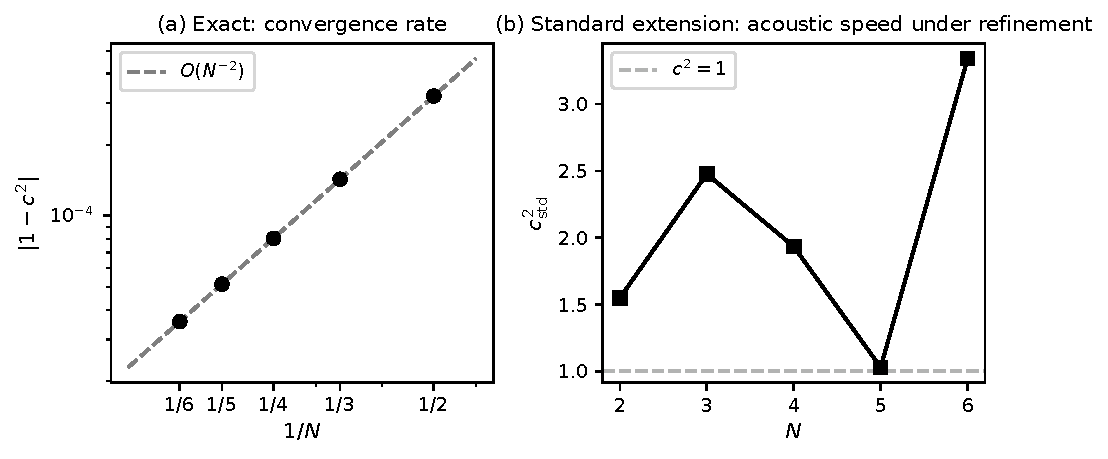
\includegraphics[width=\textwidth]{fig1_convergence_m5.pdf}
\caption{Mesh convergence of the acoustic wave speed (Kelvin foam, $5\%$~BZ along $[100]$). (a)~Exactness-preserving construction: the error $|1 - c^2|$ decreases as $O(1/N^2)$ on a log--log plot ($p = 2.00$, dashed line). (b)~Standard construction: $c^2_{\mathrm{std}}$ oscillates with increasing amplitude under refinement and does not approach the continuum value $c^2 = 1$ (dashed line).}
\label{fig:convergence}
\end{figure}

The exactness-preserving construction yields $c^2$ that converges monotonically to the correct continuum value. The error $|1 - c^2|$ decreases as $O(1/N^2)$ over the tested range (Figure~\ref{fig:convergence}a), consistent with second-order convergence typical of lowest-order structure-preserving discretizations on exact subcomplexes~\cite{Arnold2006}. The standard construction oscillates with increasing amplitude ($|\Delta c^2_{\mathrm{std}}|$ grows from $0.5$ to $2.3$ over the tested range) and does not exhibit convergence under mesh refinement. The exact construction also preserves acoustic degeneracy (modes 0 and~1 identical to machine precision), while the standard construction breaks it at all refinement levels. Voronoi $h$-refinement (random seeds, 50--350 cells per unit cell, 5 realizations each) confirms $O(h^2)$ convergence with $R^2 = 0.98$ on irregular meshes; the standard construction does not converge on these meshes either.

\subsection{Hodge splitting}
\label{sec:hodge}

The discrete Hodge decomposition of 1-forms into gradient and curl subspaces requires $\operatorname{im}(d_0) \perp \ker(d_1^\dagger\star_2)$, which follows from $d_1\,d_0 = 0$. We test this by computing the full Hodge Laplacian $\Delta_1 = K_{\mathrm{grad}} + K_{\mathrm{curl}}$ and projecting each eigenvector onto $\operatorname{im}(d_0)$.

\begin{table}[h]
\centering
\begin{tabular}{lcc}
\toprule
& Exact $d_1(\mathbf{k})$ & Standard $d_1^{\mathrm{std}}(\mathbf{k})$ \\
\midrule
Pure gradient modes & 96 & 5--23 \\
Pure curl modes & 96 & 0--7 \\
Mixed modes & 0 & 162--187 \\
\midrule
Total & 192 & 192 \\
\bottomrule
\end{tabular}
\caption{Hodge splitting of the full Hodge Laplacian eigenvectors on the Kelvin foam ($|E|{=}192$) at $5$--$10\%$ BZ. A mode is classified as ``pure'' if its projection onto $\operatorname{im}(d_0)$ is $> 0.99$ or $< 0.01$, and ``mixed'' otherwise. The exactness-preserving construction achieves perfect separation; the standard construction mixes $85$--$97\%$ of modes.}
\label{tab:hodge}
\end{table}

With the exactness-preserving $d_1(\mathbf{k})$, every eigenvector of~$\Delta_1$ is either purely gradient ($\|P_{\mathrm{grad}}\mathbf{u}\|/\|\mathbf{u}\| = 1.000$) or purely curl ($= 0.000$), with zero mixed modes out of~192. The standard construction produces 85--97\% mixed modes---nearly every eigenvector is a gradient--curl mixture.

This explains the spectral pollution structurally: in the absence of exactness, gradient modes are no longer annihilated by the curl operator and acquire a curl component through the broken Hodge splitting, making them visible to the curl--curl eigenvalue problem as spurious modes.

\subsection{Band structure}
\label{sec:bandstructure}

Figure~\ref{fig:bandstructure} shows the full band structure along the standard cubic Brillouin zone path $\Gamma$--$X$--$M$--$R$--$\Gamma$ for the Kelvin foam ($N{=}2$, $|V|{=}96$, $|E|{=}192$). The exactness-preserving construction~(a) produces clean, well-separated bands with the expected twofold acoustic degeneracy at~$\Gamma$ (blue lines). The standard construction~(b) produces dense spurious bands that collapse toward zero near every high-symmetry point, rendering the band structure severely contaminated. At~$\Gamma$ itself ($\mathbf{k} = \mathbf{0}$), both constructions coincide because $d_1^{\mathrm{std}}(\mathbf{0}) = d_1$; the pollution appears as soon as $\mathbf{k} \neq \mathbf{0}$. Panel~(c) confirms that the failure is algebraic, not numerical: $\|d_1^{\mathrm{std}}(\mathbf{k})\,d_0(\mathbf{k})\| \sim 10^{1}$ everywhere along the path, while $\|d_1^{\mathrm{exact}}(\mathbf{k})\,d_0(\mathbf{k})\| \sim 10^{-16}$ (machine precision).

\begin{figure}[h]
\centering
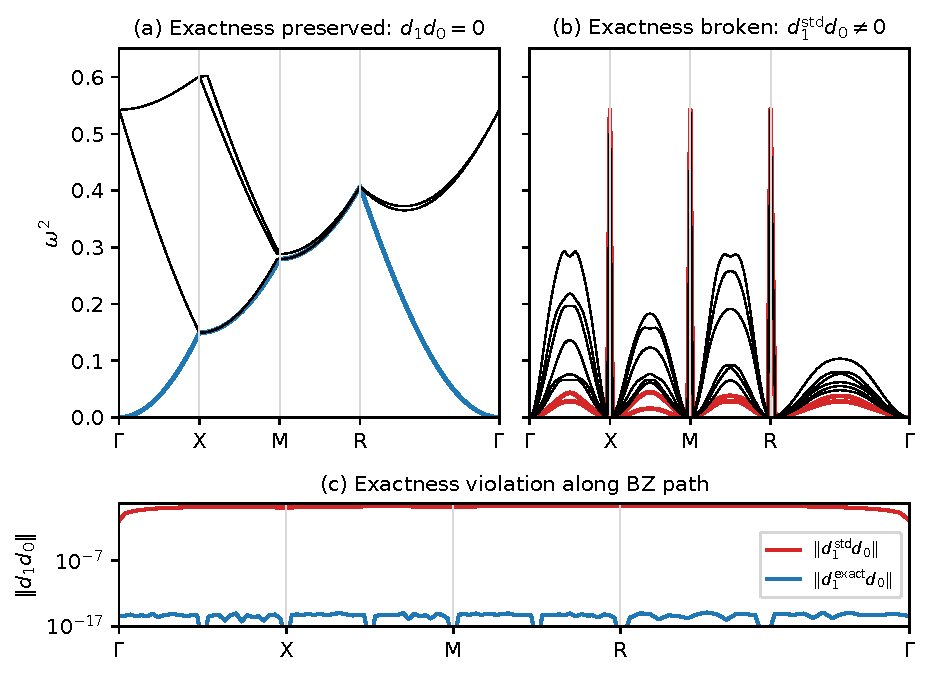
\includegraphics[width=\textwidth]{fig2_bandstructure_m5.pdf}
\caption{Band structure along $\Gamma$--$X$--$M$--$R$--$\Gamma$ for the Kelvin foam ($N{=}2$, $|V|{=}96$, $|E|{=}192$, 121~$\mathbf{k}$-points). (a)~Exactness-preserving $d_1(\mathbf{k})$: clean bands with twofold acoustic degeneracy (blue). (b)~Standard $d_1^{\mathrm{std}}(\mathbf{k})$: spurious bands (red, black) collapse toward zero; band structure is severely contaminated. (c)~Exactness violation $\|d_1\,d_0\|$ along the path: the standard construction has $O(10^1)$ violation (red), while the exact construction maintains $\|d_1\,d_0\| < 10^{-15}$ (blue) at every $\mathbf{k}$-point.}
\label{fig:bandstructure}
\end{figure}

\subsection{Universality}
\label{sec:universality}

The phenomena described above are universal across all tested structures:

\begin{table}[h]
\centering
\begin{tabular}{lccccc}
\toprule
Structure & $\|d_1^{\mathrm{std}} d_0\|$ & $n_{\mathrm{spur}}$ & $c^2_{\mathrm{exact}}$ & $c^2_{\mathrm{std}}$ & Leakage \\
\midrule
SC $N{=}3$     & 6.2  & 5      & 1.000 & ---   & ---  \\
Kelvin $N{=}2$ & 7.5  & 6--14  & 0.999 & 1.48  & 0.88 \\
C15 $N{=}1$    & 7.8  & 9--16  & 0.999 & 0.52  & 0.91 \\
WP $N{=}1$     & 5.1  & 3--7   & 0.999 & 1.20  & 0.92 \\
Random (10 seeds) & 9--12 & 12--20 & 0.998 & 0.43--1.06 & 0.88--0.91 \\
\bottomrule
\end{tabular}
\caption{Universality of exactness failure and its consequences at $10\%$ BZ. The column ``Leakage'' gives the mean gradient projection $\|P_{\mathrm{grad}}\mathbf{u}\|/\|\mathbf{u}\|$ of the spurious modes in the standard construction. All exactness-preserving results have $\|d_1 d_0\| < 10^{-15}$, $n_{\mathrm{spur}} = 0$, and leakage~$= 0$. (SC cubic: $c^2_{\mathrm{std}}$ and leakage omitted because the uniform Hodge stars on a regular lattice make $c^2_{\mathrm{exact}} = 1$ by symmetry, not by convergence; the metric quantities are not directly comparable with those on the Voronoi foams.)}
\label{tab:universality}
\end{table}

Three additional observations:
\begin{itemize}
  \item \emph{Extensive pollution.} The number of spurious modes grows with system size: $n_{\mathrm{spur}} = 6$ at $N{=}2$ ($|V|{=}96$), $17$ at $N{=}3$ ($|V|{=}324$) for the Kelvin foam along $[100]$. The pollution is not a fixed topological defect but scales with the mesh.
  \item \emph{Specific to cochain level $1{\to}2$.} The scalar Laplacian $K_0 = d_0^\dagger \star_1\,d_0$ (acting on 0-forms) has a clean spectrum with no spurious modes. The gradient $d_0(\mathbf{k})$ is uniquely defined and involves no exactness ambiguity. The pollution arises specifically at the curl level, where $d_1(\mathbf{k})$ must satisfy $d_1 d_0 = 0$.
  \item \emph{Onset at minimal supercell.} On the minimal SC cubic complex ($|V|{=}1$, $|E|{=}3$, $|F|{=}3$), each face is a square with two pairs of opposite edges carrying equal lattice shifts---a tensor-product topology where pairwise cancellation is automatic. The standard phase assignment therefore preserves exactness, and $d_1^{\mathrm{std}}(\mathbf{k})\,d_0(\mathbf{k}) = 0$. Pollution appears at the first non-trivial supercell (SC $N{=}3$: 5~spurious modes), where faces acquire boundary edges with heterogeneous shifts.
\end{itemize}

% ------------------------------------------------------------------
\section{Robustness}
\label{sec:robustness}
% ------------------------------------------------------------------

We classify perturbations into five structurally independent categories and test each on the Kelvin foam ($N{=}2$). In addition to these targeted perturbations, the spectral consequences of \S\ref{sec:consequences} were verified under: random $\mathbf{k}$-directions (23~directions including high-symmetry and generic orientations), $\mathbf{k} \to \mathbf{0}$ asymptotics ($10^{-4}$ to $20\%$~BZ), Brillouin zone boundary behavior (up to $99.9\%$~BZ), system size scaling ($N = 2, 3, 4$), 10~random Voronoi topologies, and the operator norm $\|K_{\mathrm{std}} - K_{\mathrm{exact}}\|_F$ as a function of~$|\mathbf{k}|$. In all cases, the exactness-preserving construction produces the correct kernel dimension and convergent acoustic spectrum. The failure of the standard construction is structural: it persists under refinement, random topology, random $\mathbf{k}$-directions, metric perturbations, and $\mathbf{k} \to 0$ asymptotics, and is not an artifact of insufficient resolution, special symmetry, or particular mesh choice.

Table~\ref{tab:robustness} summarizes the five targeted perturbation types. Exactness and kernel dimension are topological invariants; wave speed and degeneracy are metric and symmetry properties.

\begin{table}[h]
\centering
\begin{tabular}{llccc}
\toprule
Perturbation & Range & $d_1 d_0 = 0$ & $\ker = |V|$ & $c^2$, degeneracy \\
\midrule
Geometric (vertex positions) & $\varepsilon = 0$--$0.10$ & yes & yes & $c^2$ stable, split breaks \\
Threshold sensitivity & $10^{-8}$--$10^{-14}$ & yes & yes & unchanged \\
BZ boundary ($\mathbf{k} = \mathbf{k}_{\mathrm{BZ}}$) & $0.1$--$0.999$ BZ & yes & yes & $c^2 \to 0$ (band edge) \\
Face ordering (6 permutations) & all & yes & yes & $K$ identical \\
Gauge transform (random $\theta(v)$) & 5 seeds & yes & yes & eigenvalues identical \\
\bottomrule
\end{tabular}
\caption{Robustness summary on the Kelvin foam. Exactness and kernel dimension are preserved under all perturbation types. At the exact BZ boundary ($\mathbf{k} = \mathbf{k}_{\mathrm{BZ}}$), $\operatorname{rank}(d_0)$ drops by~1 and the kernel gains two additional zeros, but exactness is maintained and no numerical instability occurs.}
\label{tab:robustness}
\end{table}

\begin{table}[h]
\centering
\begin{tabular}{llc}
\toprule
Property & Type & Robust under \\
\midrule
$d_1(\mathbf{k})\,d_0(\mathbf{k}) = 0$ & topological & all perturbations \\
$\dim\ker K = |V|$ & topological & all perturbations \\
$\omega^2 = c^2|\mathbf{k}|^2$ & metric & geometry, symmetry \\
Polarization degeneracy & symmetry & topology, metric \\
\bottomrule
\end{tabular}
\caption{Classification of spectral properties.}
\label{tab:classification}
\end{table}

% ------------------------------------------------------------------
\section{Discussion}
\label{sec:discussion}
% ------------------------------------------------------------------

\paragraph{Relation to Boffi's exactness criterion}
Boffi~\cite{Boffi2010} showed that exactness of the discrete de~Rham complex is necessary and sufficient for spurious-free Maxwell eigenvalue computations; earlier work by Boffi, Conforti, and Gastaldi~\cite{Boffi2006} demonstrated this in the specific context of photonic crystal eigenproblems, and Dobson and Pasciak~\cite{Dobson2001} analyzed related algorithms for electromagnetic Bloch modes. Our results provide a concrete demonstration: the standard Bloch extension violates exactness on unstructured meshes, and the resulting spectral pollution, broken Hodge splitting, and convergence failure are precisely the consequences predicted by Boffi's theory. The exactness-preserving construction restores all three.

\paragraph{Connection interpretation}
The exactness violation $\|d_1^{\mathrm{std}}(\mathbf{k})\,d_0(\mathbf{k})\|$ can be interpreted as the curvature of a discrete connection. The standard Bloch extension assigns phases independently per edge, defining a connection with $O(1)$ curvature that grows with~$|\mathbf{k}|$. The curvature manifests algebraically as the non-vanishing of $d_1^{\mathrm{std}}(\mathbf{k})\,d_0(\mathbf{k})$. The recurrence construction of Theorem~\ref{thm:exact} produces a flat connection (zero curvature) by deriving all phases from those in~$d_0(\mathbf{k})$. This interpretation connects our construction to the framework of bundle-valued DEC~\cite{Braune2024}.

\paragraph{Acoustic modes and cohomological deformation}
The Betti number $\beta_1(\Gamma) = 3$ has a direct spectral interpretation. At~$\Gamma$, $M_1$-orthogonal Hodge decomposition within $\ker d_1(\mathbf{0})$ extracts three harmonic 1-forms spanning $H^1(T^3, \mathbb{C})$, separated from the 95-dimensional gradient subspace by a singular-value gap of order~$10^{13}$. At small $|\mathbf{k}| > 0$, $\beta_1(\mathbf{k}) = 0$: the harmonic subspace vanishes and all of $\ker d_1(\mathbf{k}) = \operatorname{im} d_0(\mathbf{k})$ becomes gradient. Tracking the harmonic forms via subspace trace overlaps $\operatorname{Tr}(P_H \cdot P_{\mathrm{sub}})$ gives a discrete Helmholtz decomposition:
\[
  \operatorname{Tr}(P_H \cdot P_{\mathrm{grad}}) = 1, \quad
  \operatorname{Tr}(P_H \cdot P_{\mathrm{acou}}) = 2, \quad
  \operatorname{Tr}(P_H \cdot P_{\mathrm{opt}}) = 0, \quad
  \text{sum} = 3.
\]
One harmonic form becomes a longitudinal gradient mode; two become transverse acoustic modes with dispersion $\omega^2 = |\mathbf{k}|^2$ (sound speed $v_s = 1$ in natural units). No harmonic component leaks into the optical band. This $1{+}2{+}0 = 3$ splitting is universal across all test structures (Kelvin, C15, Weaire--Phelan) and all $\mathbf{k}$-directions. The standard construction cannot perform this analysis: without $d_1 d_0 = 0$, cohomology is undefined at $\mathbf{k} \neq 0$.

\paragraph{Existing discretizations}
The finite element exterior calculus (FEEC)~\cite{Arnold2006,Arnold2010} and its smoothed projection framework~\cite{Christiansen2008} provide the theoretical foundation for structure-preserving Maxwell discretizations; Hiptmair~\cite{Hiptmair2002} gives a comprehensive treatment of edge elements in this context. The discrete de~Rham (DDR) method~\cite{DiPietro2020} achieves exactness on polyhedral meshes, and the topological framework of Gross and Kotiuga~\cite{Gross2004} treats electromagnetism on complexes. The mimetic finite difference method of~\cite{Jin2025} treats Bloch conditions on structured meshes. None of these, however, addresses the specific setting of our work: Bloch-periodic DEC on unstructured polyhedral meshes. FEEC does not treat Bloch periodicity. DDR has not been formulated with Bloch boundary conditions. Mimetic FD does not handle unstructured meshes. Our construction fills this gap: it restores the discrete exact sequence $d_1\,d_0 = 0$ within the DEC framework for Bloch-periodic problems on general polyhedral complexes. We do not address the full FEEC program (commuting projections, approximation theory); the present contribution is limited to the algebraic exactness of the discrete complex. To date, Bloch-periodic band structure computations on foam-like meshes have used plane-wave expansion~\cite{Klatt2019} rather than DEC, so the exactness defect identified here is latent---it would affect any future DEC-based computation on unstructured periodic complexes, but existing published results are not invalidated.

\paragraph{Limitations}
The Hodge stars are diagonal (circumcentric dual); non-diagonal stars would require modification of the assembly but not the exactness construction. The mesh must have valid Voronoi structure; for random point sets, sufficient density is required ($\geq 50$ points per periodic box gives $> 80\%$ valid Voronoi tessellations; the remaining cases fail at the mesh generation stage due to degenerate dual geometry, not at the exactness construction). We treat only the 3D curl--curl problem; extension to 2D and to time-domain DEC is straightforward. The construction is lowest-order (piecewise-constant cochains, analogous to Whitney 0-forms); extension to higher-order DEC, where basis functions span more than one cell, would require a corresponding generalization of the face-boundary recurrence. The observed second-order convergence rate (Table~\ref{tab:convergence}) is consistent with a lowest-order discretization but a formal error estimate relating mesh size to eigenvalue error is not attempted.

\paragraph{Cross-validation against plane-wave expansion}
To assess quantitative accuracy, we compare DEC eigenvalues against MIT Photonic Bands (MPB)~\cite{Johnson2001} on a BCC Voronoi foam (Kelvin cell) with dielectric contrast $\varepsilon_A = 1$, $\varepsilon_B = 2, 4, 9$. Both methods solve the same geometry; MPB uses a voxelized approximation that converges with grid resolution ($< 0.5\%$ change from resolution~32 to~64). The DEC overestimates $c^2 = \omega^2/|\mathbf{k}|^2$ relative to MPB: $+5\%$ at $\varepsilon_B = 2$, $+21\%$ at $\varepsilon_B = 4$, $+50\%$ at $\varepsilon_B = 9$. A $\mathbf{k}$-scaling test at two wavevectors reveals two distinct error mechanisms: in vacuum, the discrepancy scales as $O(k^2)$ (dispersion error); at finite contrast, a $\mathbf{k}$-independent contribution dominates, arising from the piecewise-constant $\varepsilon$ approximation in the Hodge star. The choice of interface averaging formula---harmonic mean of $1/\varepsilon$ ($+21\%$), geometric mean ($+4\%$), or arithmetic mean of $\varepsilon$ ($-12\%$)---does not affect exactness ($n_{\mathrm{zero}} = |V|$ at all schemes) but determines quantitative accuracy. The DEC--MPB gap is entirely in the Hodge star, not in the complex.

% ------------------------------------------------------------------
\section{Conclusion}
\label{sec:conclusion}
% ------------------------------------------------------------------

The standard Bloch-periodic extension of DEC does not preserve the discrete exact sequence on unstructured polyhedral meshes. This structural inconsistency produces spectral pollution that enters the physical spectrum, compromises the discrete Hodge decomposition, and mesh convergence of the acoustic wave speed is not observed under refinement in the tested regime. A face-boundary recurrence restores exactness by deriving the curl phases from those already present in the gradient, producing a canonical curl--curl operator with correct gauge kernel and acoustic spectrum. The exact complex computes the twisted de~Rham cohomology $H^*(T^3, \mathcal{L}_\mathbf{k})$ with the correct Betti numbers, and the Helmholtz decomposition $1{+}2{+}0 = 3$ connects the cohomological invariants at~$\Gamma$ to the acoustic band structure at small~$|\mathbf{k}|$. The failure is algebraic---it is independent of mesh quality, resolution, or symmetry---and persists under refinement. Verification on simple cubic, Voronoi foam, and random Voronoi complexes confirms that the construction is universal and robust.

% ------------------------------------------------------------------
\section*{Reproducibility}
% ------------------------------------------------------------------

All computations use Python~3.9, NumPy, SciPy (LAPACK/BLAS). Source code and a structured test suite are available at \url{https://github.com/alex-toader/st_bloch_exactness}. The test suite covers exactness verification, spectral pollution counts, kernel dimension, $\mathbf{k} \to 0$ asymptotics, random $\mathbf{k}$-directions, Brillouin zone boundary behavior, mesh refinement convergence, random Voronoi topologies, operator perturbation norms, full Hodge Laplacian splitting, face ordering independence, twisted cohomology computation, harmonic form extraction, and Helmholtz decomposition verification. All numerical claims in this paper are backed by reproducible scripts.

% ------------------------------------------------------------------
\bibliographystyle{elsarticle-num}

\begin{thebibliography}{99}

\bibitem{Arnold2006}
D.N.~Arnold, R.S.~Falk, R.~Winther,
Finite element exterior calculus, homological techniques, and applications,
\emph{Acta Numerica} 15 (2006) 1--155.

\bibitem{Arnold2010}
D.N.~Arnold, R.S.~Falk, R.~Winther,
Finite element exterior calculus: from Hodge theory to numerical stability,
\emph{Bull.\ Amer.\ Math.\ Soc.} 47 (2010) 281--354.

\bibitem{Boffi2010}
D.~Boffi,
Finite element approximation of eigenvalue problems,
\emph{Acta Numerica} 19 (2010) 1--120.

\bibitem{Boffi2006}
D.~Boffi, M.~Conforti, L.~Gastaldi,
Modified edge finite elements for photonic crystals,
\emph{Numer.\ Math.} 105 (2006) 249--266.

\bibitem{Bott1982}
R.~Bott, L.W.~Tu,
\emph{Differential Forms in Algebraic Topology},
Springer, 1982.

\bibitem{Braune2024}
T.~Braune, Y.~Tong, F.~Gay-Balmaz, M.~Desbrun,
A discrete exterior calculus of bundle-valued forms,
arXiv:2406.05383, 2024.

\bibitem{Chen2017}
S.C.~Chen, W.C.~Chew,
Numerical electromagnetic frequency domain analysis with discrete exterior calculus,
\emph{J.\ Comput.\ Phys.} 350 (2017) 668--689.

\bibitem{Christiansen2008}
S.H.~Christiansen, R.~Winther,
Smoothed projections in finite element exterior calculus,
\emph{Math.\ Comp.} 77 (2008) 813--829.

\bibitem{Desbrun2005}
M.~Desbrun, A.N.~Hirani, M.~Leok, J.E.~Marsden,
Discrete exterior calculus,
arXiv:math/0508341, 2005.

\bibitem{DiPietro2020}
D.A.~Di~Pietro, J.~Droniou,
\emph{The Hybrid High-Order Method for Polytopal Meshes},
Springer, 2020.

\bibitem{Dobson2001}
D.C.~Dobson, J.E.~Pasciak,
Analysis of an algorithm for computing electromagnetic Bloch modes using Nedelec spaces,
\emph{Comput.\ Methods Appl.\ Math.} 1 (2001) 138--153.

\bibitem{Gross2004}
P.W.~Gross, P.R.~Kotiuga,
\emph{Electromagnetic Theory and Computation: A Topological Approach},
Cambridge University Press, 2004.

\bibitem{Hiptmair2002}
R.~Hiptmair,
Finite elements in computational electromagnetism,
\emph{Acta Numerica} 11 (2002) 237--339.

\bibitem{Hirani2003}
A.N.~Hirani,
\emph{Discrete Exterior Calculus},
PhD thesis, Caltech, 2003.

\bibitem{Jin2025}
C.~Jin, Y.~Xia, Y.~Xu,
Kernel compensation method for Maxwell eigenproblem in photonic crystals with mimetic finite difference discretizations,
\emph{Numer.\ Methods Partial Differ.\ Eq.} 41 (2025) e23171.

\bibitem{Klatt2019}
M.A.~Klatt, P.J.~Steinhardt, S.~Torquato,
Phoamtonic designs yield sizeable 3D photonic band gaps,
\emph{PNAS} 116 (2019) 23480--23486.

\bibitem{Teixeira1999}
F.L.~Teixeira, W.C.~Chew,
Lattice electromagnetic theory from a topological viewpoint,
\emph{J.\ Math.\ Phys.} 40 (1999) 169--187.

\end{thebibliography}

\section*{Declaration of generative AI and AI-assisted technologies in the manuscript preparation process}

During the preparation of this work the author used Claude (Anthropic) in order to assist with code review, test suite consolidation, and manuscript formatting. After using this tool, the author reviewed and edited the content as needed and takes full responsibility for the content of the published article.

\end{document}
